\documentclass[letterpaper]{amsart}
\usepackage{times}
\usepackage{tikz}
\usepackage{calc}
\usetikzlibrary{arrows.meta}

\title[Homework 2]{Homework 2 \\ OR647: Queueing Theory, Spring 2021}
\author{David Prentiss}
\email{dprentis@gmu.edu}
\date{\today}

\begin{document}
\maketitle

\section{} %1
A cloud computing service is modeled as a fluid queue with time-dependent
arrival rate $\lambda(t)$ and constant service rate $\mu$. Consider a situation where the
arrival process has a burst. Initially, the arrival rate is $\lambda_1<\mu$. Then, for a
period of length $T$, the arrival process is $\lambda_2>\mu$, after which it
returns back to $\lambda_1$.

\subsection*{a}
What is the maximum queue length?
\subsubsection*{Solution}
Let the burst begin at time $t_0 = 0$ and end at $t_T = T$. For times $t<t_0$, the
cumulative number of arrivals, $A(t)$, equals the cumulative number of
departures, $D(t)$, since $\lambda(t) = \lambda_1 < \mu$. Therefore the queue
length $L$ is zero. For times $t_0\leq t<t_T$ however, $\lambda(t) = t_2 > \mu$
and cumulative arrivals are greater than cumulative departures. We also know
that the queue length at time $t$, $L(t)$, is the difference $A(t)-D(t)$.
Furthermore, the moment when the queue length is greatest is $t_T$. This follows
from the fact that the queue length is increasing from $t_0$ to $t_T$ and begins
decreasing at time $t_T$. So then,
\begin{align*}
  L_\text{max} &= A(t_T) - D(t_T) \\
  &= \int_{t_0}^{t_T}\lambda(t)dt - \int_{t_0}^{t_T}\mu dt + A(t_0)-D(t_0) \\
  &= T(\lambda_2 - \mu).
\end{align*}

\subsection*{b}
What is the length of the busy period (i.e., the time from the start of the burst until the
queue empties)?

\subsubsection*{Solution}
Let $T_e$ be the length of time from $t_T$ to the end of the busy period, $t_e$. We know the
queue length at $t=t_T$ and we know the queue empties at rate $(\mu-\lambda_1)$.
\begin{align*}
  T_e(\mu - \lambda_1) &= T(\lambda_2 - \mu) \\
  T_e &= \frac{T(\lambda_2 - \mu)}{\mu - \lambda_1}.
\end{align*}
So the total busy period, $T_b$, is
\begin{align*}
  T_b &= T + T_e \\
  &= T + \frac{T(\lambda_2 - \mu)}{\mu-\lambda_1} \\
      &= \frac{T(\mu-\lambda_1)}{\mu-\lambda_1} + \frac{T(\lambda_2 - \mu)}{\mu-\lambda_1} \\
  &=\frac{T(\lambda_2-\lambda_1)}{\mu-\lambda_1}
\end{align*}

\subsection*{c}
What is the total delay (among all jobs) due to the burst?

\subsubsection*{Solution}
Find $\int_TA(t)-D(t)+\int_{T_e}A(t)-D(t)$ geometrically.
\begin{equation*}
  \frac{1}{2}T^2(\lambda_2-\mu)\left( \frac{\lambda_2-\lambda_1}{\mu-\lambda_1} \right)
\end{equation*}

\section{} %2
A road segment is modeled as a fluid queue. The arrival rate is shown in the graph below,
with a morning rush hour. After the morning rush hour, the transportation department
begins maintenance work on the road. At 9 a.m., one of the three lanes on the road is
closed, reducing the capacity of the road from 15 cars per minute to 10 cars per minute.
The maintenance period ends at noon.
\subsection*{d}
Determine the average delay per car (over all cars from 6 a.m.to 1 p.m.).
\subsubsection*{Solution}
Calculate the area of $A(t) - D(t)$ (193,500) geometrically and divide by the total number
of vehicle arrivals in the time period (2400) to find the average delay of 41.61 minutes.
\begin{center}
\begin{tabular}{rccccc}
  time, $t$ (min) & 60 & 120 & 180 & 360 & 390(f)\\
  $\lambda(t)$ (veh/min)&10& 20& 30& 5& 5\\
  $D^\prime(t)$ (veh/min)&10& 15& 15& 10& 15 \\
  $A(t)$ (veh) &600& 1800 & 3600 & 4500& 4650 \\
  $D(t)$ (veh) &600& 1500 & 2400(e)& 4200& 4650 \\
  Queue length (veh) &0&  300& 1200& 300&    0 \\
  %$\int A(t)-D(t)$ (veh$\cdot$hr)&0&150 & 900 & 3150 & 3225 \\
  Total delay (veh$\cdot$min)& 0 & 9000 & 54000 & 189000 & 193500\\
  Average delay (min) & 0.0 & 5.0 & 15.0 & 42.0 & 41.61(d)
\end{tabular}
\end{center}
\subsection*{e}
What is the maximum length of the queue over this period?
\subsubsection*{Solution}
Calculate the $A(t)-D(t)$ iteratively from $t=0$ and choose the largest value (1200 vehicles).
\subsection*{f}
At what time does the queue length return to 0?
\subsubsection*{Solution}
Find the intersection of $A(t)$ and $D(t)$ geometrically to find 390 minutes
elapesed time (12:30 p.m.).

\section{Problem 8.12} %3
Airplanes arrive at an airport at a rate of 30 per hour. The arrival capacity
of the airport is 40 airplanes per hour during good weather. During periods
of fog, the arrival capacity drops to 20 airplanes per hour. Suppose that the
airport experiences fog from 8 am to 10 am. Using a fluid approximation,
and considering only arrivals between 8 am and noon, what is the average
delay for each airplane?

\subsubsection*{Solution}
Solve geometrically as before.
10 minutes.

\section{Problem 8.17} %4
A traffic signal has a left-hand turn lane. The signal alternates from a red
light to a green left-hand turn arrow (cars can turn left) to a solid green light
(cars can turn left but must yield to oncoming traffic). Cars flow through
the signal at a rate of 15 per minute when there is a left-hand arrow, but
only 10 per minute when there is a regular green light. The signal spends
2 min in red, 1 min as a green left-hand arrow, and 1 min as a green light.
The arrival rate of cars who want to turn left is 6 per minute. Under a fluid
approximation, what is the average time spent waiting to turn left?
\subsubsection*{Solution}
Solve geometrically as before.
23 minutes

\section{Problem 8.18} %5
The following diagram shows a freeway on-ramp. The maximum rate that
cars can pass through point A is 60 per minute. Due to a stop light at B, the
in-flow of cars to the freeway comes in waves. The stop light is ``off'' for
2 min (during which no cars enter the freeway) and ``on'' for 1 min, during
which cars enter the freeway at a rate of 30 per minute. During periods of
congestion at A, assume that up to half of the flow-rate is applied to cars
arriving from B (i.e., cars merge on a one-to-one basis).
\subsection*{a}
What is the maximum flow rate of cars through point C that maintains
stability of the system?
\subsubsection*{Solution}
The average flow from B in one cycle is $30 /(1+2)=10\text{ veh/min}$. So the
maximum stable flow from A is $60-10=50\text{ veh/min}$.
\subsection*{b}
Assume that the flow rate of cars through C is 45 per minute. Using a
fluid approximation, what is the average delay per car on the freeway
due to the on-ramp?
\subsubsection*{Solution}
During the ``on'' phase the departure rate is 30 veh/min (60/2) otherwise it may
be as high as 60 veh/min. We assume congestion is cleared which means we will
consider the one-minute ``on'' phase first to accumulate congestion.
Solving geometrically as before. 5 seconds.
\subsection*{c}
What is the average delay per car on the on-ramp?
\subsubsection*{Solution}
This time, we begin with the ``off'' phase.
Assume the arrival rate is constant (10 veh/min).
Solving geometrically as before. 20 seconds.


\section{Problem 2.12} %6
A certain software company has a technical support line. Requests for
technical support arrive according to a Poisson process with rate
$\lambda=20\text{ per hour}$ hour. What is the probability that:
\subsection*{a}
No calls arrive during 1 hour?
\subsubsection*{Solution}
\begin{equation*}
  \text{Pr}\{N(1)=0\}=e^{-20\cdot 1}\frac{(20\cdot 1)^0}{0!} =e^{-20}
  \approx 2.061\times 10^{-9}
\end{equation*}
\subsection*{b}
Exactly 5 calls arrive during 1 hour?
\subsubsection*{Solution}
\begin{equation*}
\text{Pr}\{N(1)=5\}=e^{-20\cdot 1}\frac{(20\cdot 1)^5}{5!}\approx 5.496\times 10^{-5}
\end{equation*}
\subsection*{c}
5 or more calls arrive during 1 hour?
\subsubsection*{Solution}
\begin{equation*}
\begin{aligned}
\text{Pr}\{N(1)\geq 5\}&=
1 - \text{Pr}\{N(1)\leq 4\}=
1-e^{-20\cdot 1}\sum_{i=0}^4\frac{(20\cdot 1)^i}{i!} \\
&\approx 0.99998
\end{aligned}
\end{equation*}

\section{Problem 2.13} %7
The following diagram represents a continuous-time Markov chain (where
the numbers represent transition rates $q_{ij}$). Find the fraction of time the
chain spends in each state.
\begin{figure}[!h]
  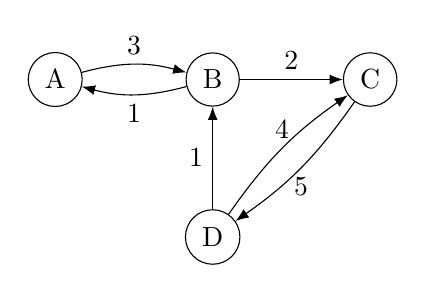
\begin{tikzpicture}[node distance={2cm}, state/.style = {draw, circle}]
    \node[state] (A) {A};
    \node[state] (B) [right of=A] {B};
    \node[state] (C) [right of=B] {C};
    \node[state] (D) [below of=B] {D};

    \path[-Latex] (A) edge[bend left=15] node[above] {3} (B);
    \draw[-Latex] (B) edge[bend left=15] node[below] {1} (A);
    \draw[-Latex] (B) edge node[above] {2} (C);
    \draw[-Latex] (D) edge node[left] {1} (B);
    \draw[-Latex] (C) edge[bend left=10] node[below] {5} (D);
    \draw[-Latex] (D) edge[bend left=10] node[above] {4} (C);
  \end{tikzpicture}
\end{figure}

\subsubsection*{Solution}
\begin{equation*}
  \{q_{ij}\}=
\begin{bmatrix}
  0 & 3 & 0 & 0 \\
  1 & 0 & 2 & 0 \\
  0 & 0 & 0 & 5 \\
  0 & 1 & 4 & 0
\end{bmatrix}
\end{equation*}

\begin{equation*}
  \{v_i\}=
  \{q_{ij}\}J_{j,1} =
\begin{bmatrix}
  0 & 3 & 0 & 0 \\
  1 & 0 & 2 & 0 \\
  0 & 0 & 0 & 5 \\
  0 & 1 & 4 & 0
\end{bmatrix}
\begin{bmatrix}
  1 \\ 1 \\ 1 \\ 1
\end{bmatrix}
=
\begin{bmatrix}
  3 \\ 3 \\ 5 \\ 5
\end{bmatrix}
\end{equation*}
\begin{equation*}
\mathbf{Q}=
\begin{bmatrix}
  -3 & 3 & 0 & 0 \\
  1 & -3 & 2 & 0 \\
  0 & 0 & -5 & 5 \\
  0 & 1 & 4 & -5
\end{bmatrix}
\end{equation*}
The fraction of time spent in each state are the stationary probabilities.
\begin{align*}
  \mathbf{0} &=\vec{p}\mathbf{Q}
               \land
  \sum_ip_i=1\\
\begin{bmatrix}
  \left[\mathbf{Q}\right]^\mathsf{T} \\
  J_{1,j}
\end{bmatrix}
  \vec{p} &=
              \begin{bmatrix}
                \mathbf{0} \\
                1
              \end{bmatrix}
  \\
  \vec{p} &=
\begin{bmatrix}
  \frac{1}{16} &
  \frac{3}{16} &
  \frac{3}{8} &
  \frac{3}{8}
\end{bmatrix}
\end{align*}

\section{Problem 2.15} %8
Customers arrive at a shuttle stop according to a Poisson process with rate 3
per hour. Shuttles arrive at the stop according to a Poisson process with
rate 1.5 per hour. Suppose that each shuttle can hold at most 2 customers.
Suppose that at most 4 people wait for the shuttle (subsequently arriving
customers are turned away).
\subsection*{a}
 Model this process as a continuous-time Markov chain. Give the rate
 transition matrix $\mathbf{Q}$.
\subsubsection*{Solution}
Assume arriving shuttles are empty.
\begin{equation*}
  \{q_{ij}\}=
\begin{bmatrix}
  0 & 3 & 0 & 0 & 0 \\
  1.5 & 0 & 3 & 0 & 0 \\
  1.5 & 0 & 0 & 3 & 0 \\
  0 & 1.5 & 0 & 0 & 3 \\
  0 & 0 & 1.5 & 0 & 0
\end{bmatrix}
\end{equation*}
\begin{equation*}
  \{v_i\}=
  \{q_{ij}\}J_{j,1} =
\begin{bmatrix}
  3 \\ 4.5 \\ 4.5 \\ 4.5 \\ 1.5
\end{bmatrix}
\end{equation*}
\begin{equation*}
  \mathbf{Q} =
\begin{bmatrix}
  -3 & 3 & 0 & 0 & 0 \\
  1.5 & -4.5 & 3 & 0 & 0 \\
  1.5 & 0 & -4.5 & 3 & 0 \\
  0 & 1.5 & 0 & -4.5 & 3 \\
  0 & 0 & 1.5 & 0 & -1.5
\end{bmatrix}
\end{equation*}
\subsection*{b}
Give the probability transition matrix $\mathbf{P}$ of the embedded discrete-time
Markov chain.
\subsubsection*{Solution}
\begin{equation*}
  \mathbf{P} =
\begin{bmatrix}
  0 & 1 & 0 & 0 & 0 \\
  \frac{1}{3} & 0 & \frac{2}{3} & 0 & 0 \\
  \frac{1}{3} & 0 & 0 & \frac{2}{3} & 0 \\
  0 & \frac{1}{3} & 0 & 0 & \frac{2}{3} \\
  0 & 0 & 1 & 0 & 0
\end{bmatrix}
\end{equation*}
\subsection*{c}
Solve for the stationary probabilities $p_i$ (of the CTMC) and $\pi_i$ (of the
embedded DTMC).
\subsubsection*{Solution}
For the CTMC
\begin{align*}
  \mathbf{0} &=\vec{p}\mathbf{Q}
               \land
  \sum_ip_i=1\\
\begin{bmatrix}
  \left[\mathbf{Q}\right]^\mathsf{T} \\
  J_{1,j}
\end{bmatrix}
  \vec{p} &=
              \begin{bmatrix}
                \mathbf{0} \\
                1
              \end{bmatrix}
  \\
  \vec{p} &=
\begin{bmatrix}
  \frac{11}{57} &
  \frac{10}{57} &
  \frac{4}{19} &
  \frac{8}{57} &
  \frac{16}{57}
\end{bmatrix}
\end{align*}
For the embedded DTMC
\begin{align*}
  \mathbf{0} &=\vec{\pi}(\mathbf{P}-\mathbf{I})
               \land
  \sum_i\pi_i=1\\
\begin{bmatrix}
  \left[\mathbf{P}-\mathbf{I}\right]^\mathsf{T} \\
  J_{1,j}
\end{bmatrix}
  \vec{\pi} &=
              \begin{bmatrix}
                \mathbf{0} \\
                1
              \end{bmatrix}
  \\
  \vec{\pi} &=
\begin{bmatrix}
  \frac{11}{64} &
  \frac{15}{64} &
  \frac{9}{32} &
  \frac{3}{16} &
  \frac{1}{8}
\end{bmatrix}
\end{align*}
\subsection*{d}
What is the average number of customers who enter a shuttle?
\subsubsection*{Solution}
Calculate the average number of customers weighted by probabilities $\vec{p}$.

\begin{equation*}
\begin{aligned}
  \frac{11}{57}\cdot 0\text{ passengers}
  &+
  \frac{10}{57}\cdot 1\text{ passenger}
  +
  \left(
  \frac{4}{19}
  +
  \frac{8}{57}
  +
  \frac{16}{57}
  \right)\cdot 2\text{ passengers}\\
  &=
  \frac{82}{57}\text{ passengers}
  \approx 1.44\text{ passengers}
\end{aligned}
\end{equation*}


\section{Problem 3.10} %9
The following is a graph of the arrival rate of customers (over a 2-hour
period). You decide to model this as an M/M/1 queue with service rate 30
per hr. Compute the average wait in queue if you:
\subsection*{a}
Assume that the arrival rate is constant over the 2-hour period (dashed
line)
\subsubsection*{Solution}
Let
$\lambda=15/\text{h}$
and
$\mu=30/\text{hr}$,
then
$\rho=\frac{1}{2}$
and
$W_q=\frac{\rho}{\mu-\lambda}=\text{h}/30=2\text{ min}$.
\subsection*{b}
Assume that the arrival rate is constant over specific intervals (solid
line). Assume the queue is in steady state over each interval, compute
the average wait in queue for each interval and then compute the overall
average wait in queue.
\subsubsection*{Solution}
For $0<t\leq 40$ and $80<t\leq120$, let
$\lambda=10/\text{h}$
and
$\mu=30/\text{h}$,
then
$\rho=\frac{1}{3}$
and
$W_q=\frac{\rho}{\mu-\lambda}=\text{h}/60=1\text{ min}$.
For $40<t\leq 80$, let
$\lambda=25/\text{h}$
and
$\mu=30/\text{h}$,
then
$\rho=\frac{5}{6}$
and
$W_q=\frac{\rho}{\mu-\lambda}=\text{h}/6=10\text{ min}$.
The average wait time in the queue for the two-hour period is
$\frac{2}{3}\cdot 1\text{ min} + \frac{1}{3}\cdot 10\text{ min}=4\text{ min}$.

\subsection*{c}
Does the simpler model in (a) overestimate or underestimate the congestion compared with using a nonstationary model?
\subsubsection*{Solution}
As shown in parts (a) and (b) the simpler model underestimates the congestion as
compared with the nonstationary model.

\section{Problem 3.11} %10
A car rental agency has a kiosk at the airport with a single customer service
agent. Arrivals to the kiosk are Poisson with a rate of 8 per hour. The time
to process a customer is exponential with a mean time of 5 minutes.
\subsection*{a}
What is the average time that a customer spends at the kiosk (wait in
queue plus service time)?
\subsubsection*{Solution}
Let
$\lambda=8/\text{h}=\frac{2}{15}/\text{min}$
and
$\mu=\frac{1}{5}/\text{min}$,
then
\begin{equation*}
\text{E}[T]=\frac{1}{\mu-\lambda}=15\text{ min}.
\end{equation*}
\subsection*{b}
Suppose that an arriving customer will be late for a wedding if the time
spent at the kiosk is more than 20 minutes. What is the probability the
customer makes it to the wedding on time?
\subsubsection*{Solution}
$W(t) = 1-e^{-(\mu-\lambda)t}$
\begin{align*}
  \text{Pr}\{T<20\}&= W(20) \\
  &= 1-e^{-(\frac{1}{5}-\frac{2}{15})20} \\
  &= 1-e^{-(\frac{1}{15})20} \\
  &\approx 0.736
\end{align*}
\subsection*{c}
What is the probability that the customer is late to the wedding but not
less than 5 minutes late (i.e., the time spent at the kiosk is between 20
and 25 minutes)?
\subsubsection*{Solution}
\begin{align*}
\text{Pr}\{20<T<25\}&=W(25)-W(20) \\
  &= 1-e^{-(\frac{1}{15})25} -W(20)\\
  &\approx 0.075
\end{align*}
%then $\rho=\frac{2}{3}$.
%$L_q=\frac{\rho^2}{1-\rho}=\frac{4}{3}\approx 1.333$
%$L=\frac{\rho}{1-\rho}=2$

\end{document}
